\documentclass[10pt]{standalone}
\usepackage{pgfplots}
\pgfplotsset{compat=1.15}
\usepackage{mathrsfs}
\usetikzlibrary{arrows}
\pagestyle{empty}
\begin{document}
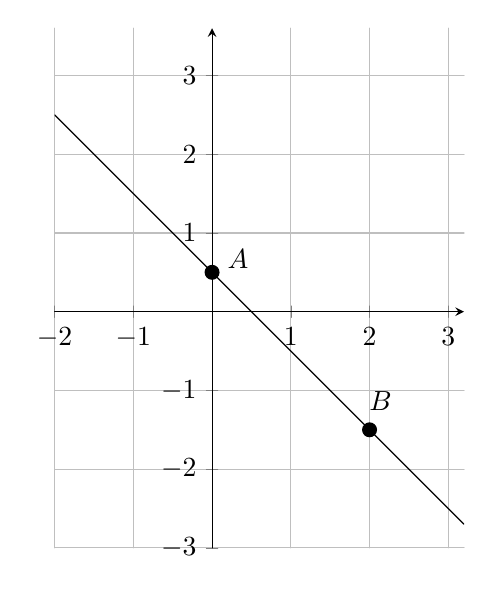
\begin{tikzpicture}[line cap=round,line join=round,>=triangle 45,x=1.0cm,y=1.0cm]
\begin{axis}[
x=1.0cm,y=1.0cm,
axis lines=middle,
ymajorgrids=true,
xmajorgrids=true,
xmin=-2.0,
xmax=3.2,
ymin=-3.0,
ymax=3.6,
xtick={-2.0,-1.0,...,3.0},
ytick={-3.0,-2.0,...,3.0},]
\clip(-2.,-3.) rectangle (3.2,3.6);
\draw [domain=-2.:3.2] plot(\x,{(--1.-2.*\x)/2.});
\begin{scriptsize}
\draw [fill=black] (0.,0.5) circle (2.5pt);
\draw [fill=black] (2.,-1.5) circle (2.5pt);
\draw[color=black] (2.14,-1.13) node {$B$};
\draw[color=black] (0.33,0.67) node {$A$};
\end{scriptsize}
\end{axis}
\end{tikzpicture}
\end{document}